\section{Getting Around -- Site Navigation}

After logging in (and performing most actions), you will be presented with a calendar view of the current month's events.

There are three different ways to see the currently booked events: by month, by week, and by day. You can switch between each view by clicking the buttons in the upper-right hand corner of the screen.


\subsection{Events}

Events are room bookings made in the name of a Storefront Partner. Events are colour coded according to their status: tentative (blue), confirmed (green), or rejected (red). Only Administrator-level users can make confirmed bookings, or change booking statuses. All other user levels may only create tentative (requested) events.


\subsection{Navigation by Month}

This is the default view that you will see after logging in. By default, the month presented is the current month. To view a different month, navigate backwards and forwards using the arrow buttons in the upper-left corner.

Tip: If you are an Administrator, you can drag-and-drop events to different days. You can also confirm a tentative booking by single left-clicking on it.

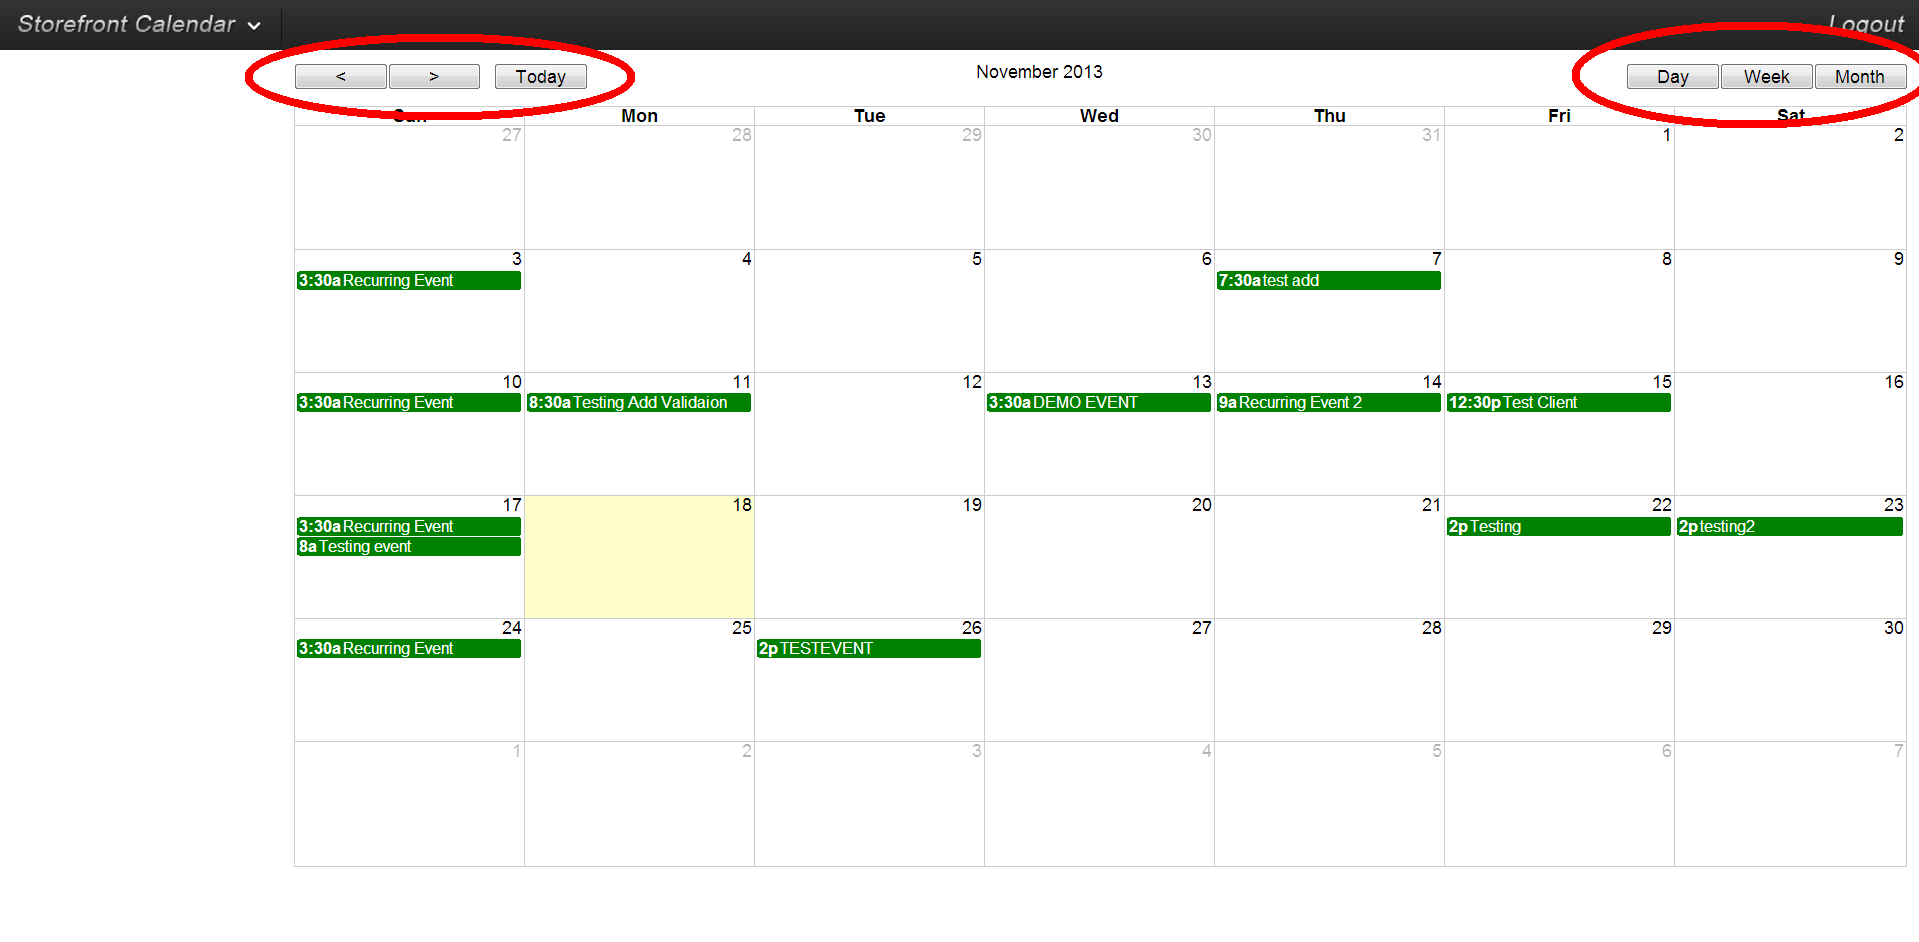
\includegraphics[width=\linewidth]{screenshots/img_month}

\newpage


\subsection{Navigation by Week}

In this view, the columns are days of the week, and the rows are booking times. By default, the week presented is the current week. To view a different week, navigate backwards and forwards using the arrow buttons.

Tip: If you are an Administrator, you can drag-and-drop events to different days and times. You can also confirm a tentative booking by single left-clicking on it.

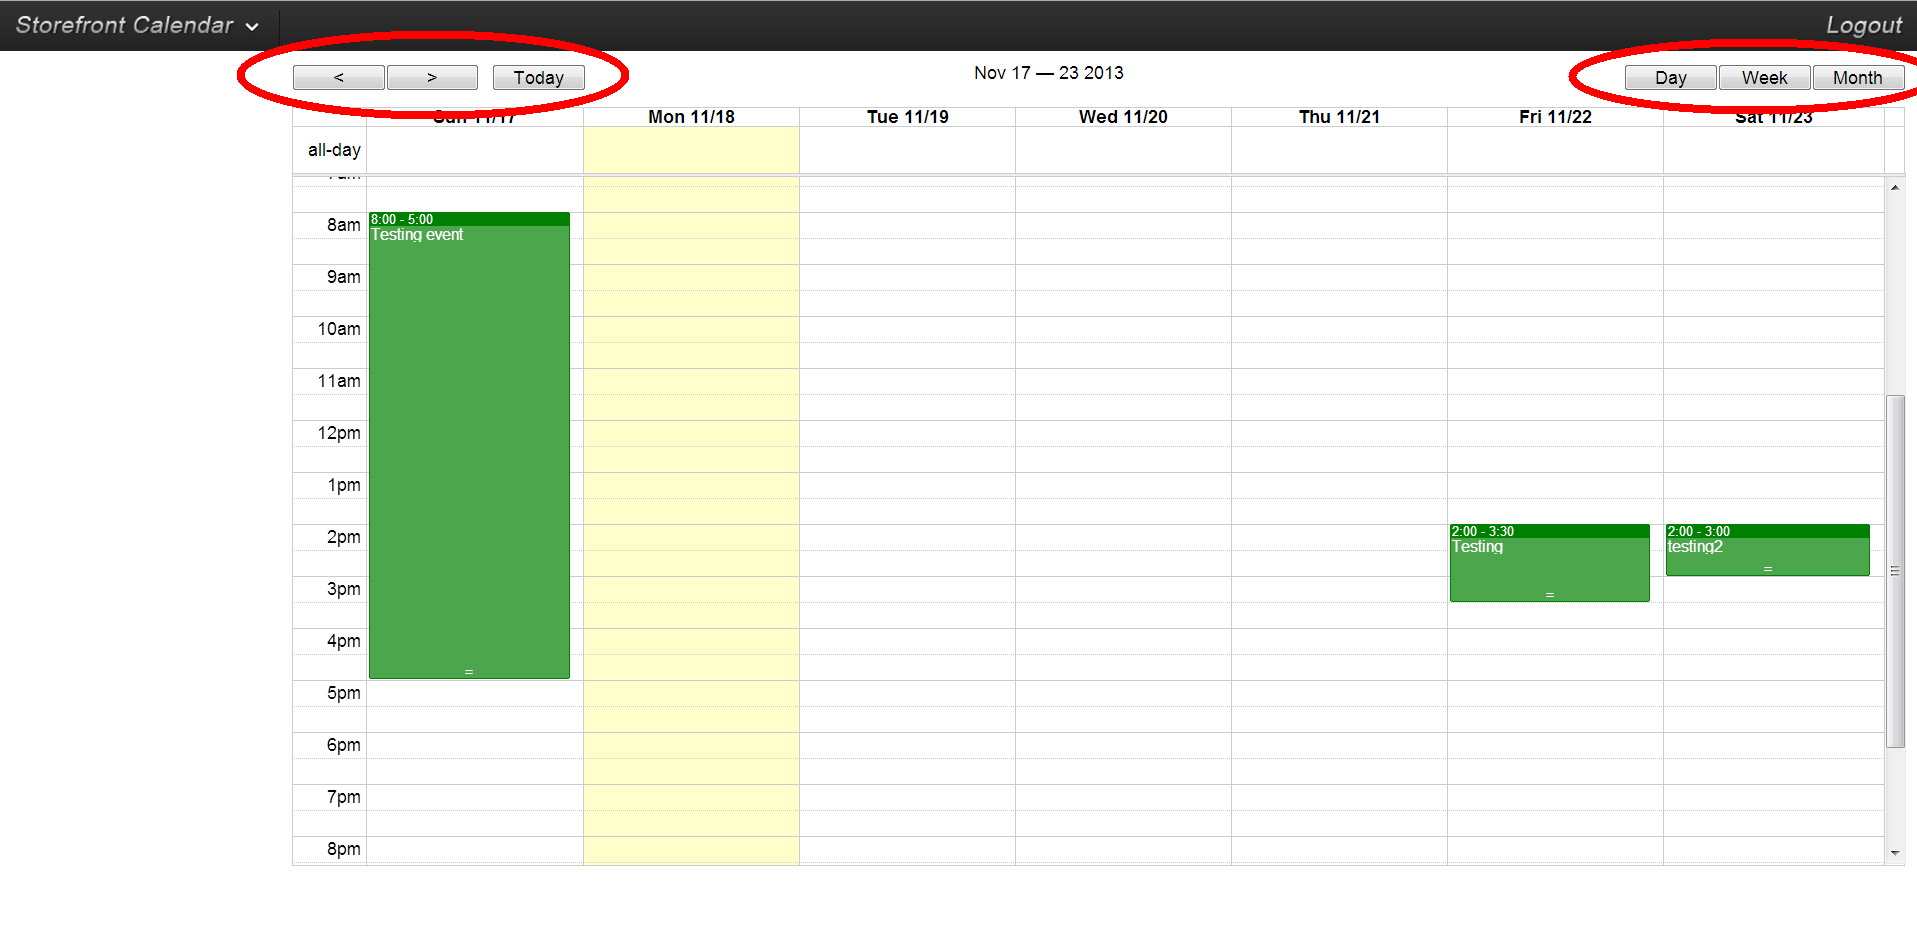
\includegraphics[width=\linewidth]{screenshots/img_week}


\newpage


\subsection{Navigation by Day}

The columns are bookable rooms, and the rows are booking times. By default, the day presented is the current day. To view a different day, navigate backwards and forwards using the arrow buttons.

Tip: If you are an Administrator, you can drag-and-drop events to different times and rooms. You can also confirm a tentative booking by single left-clicking on it.

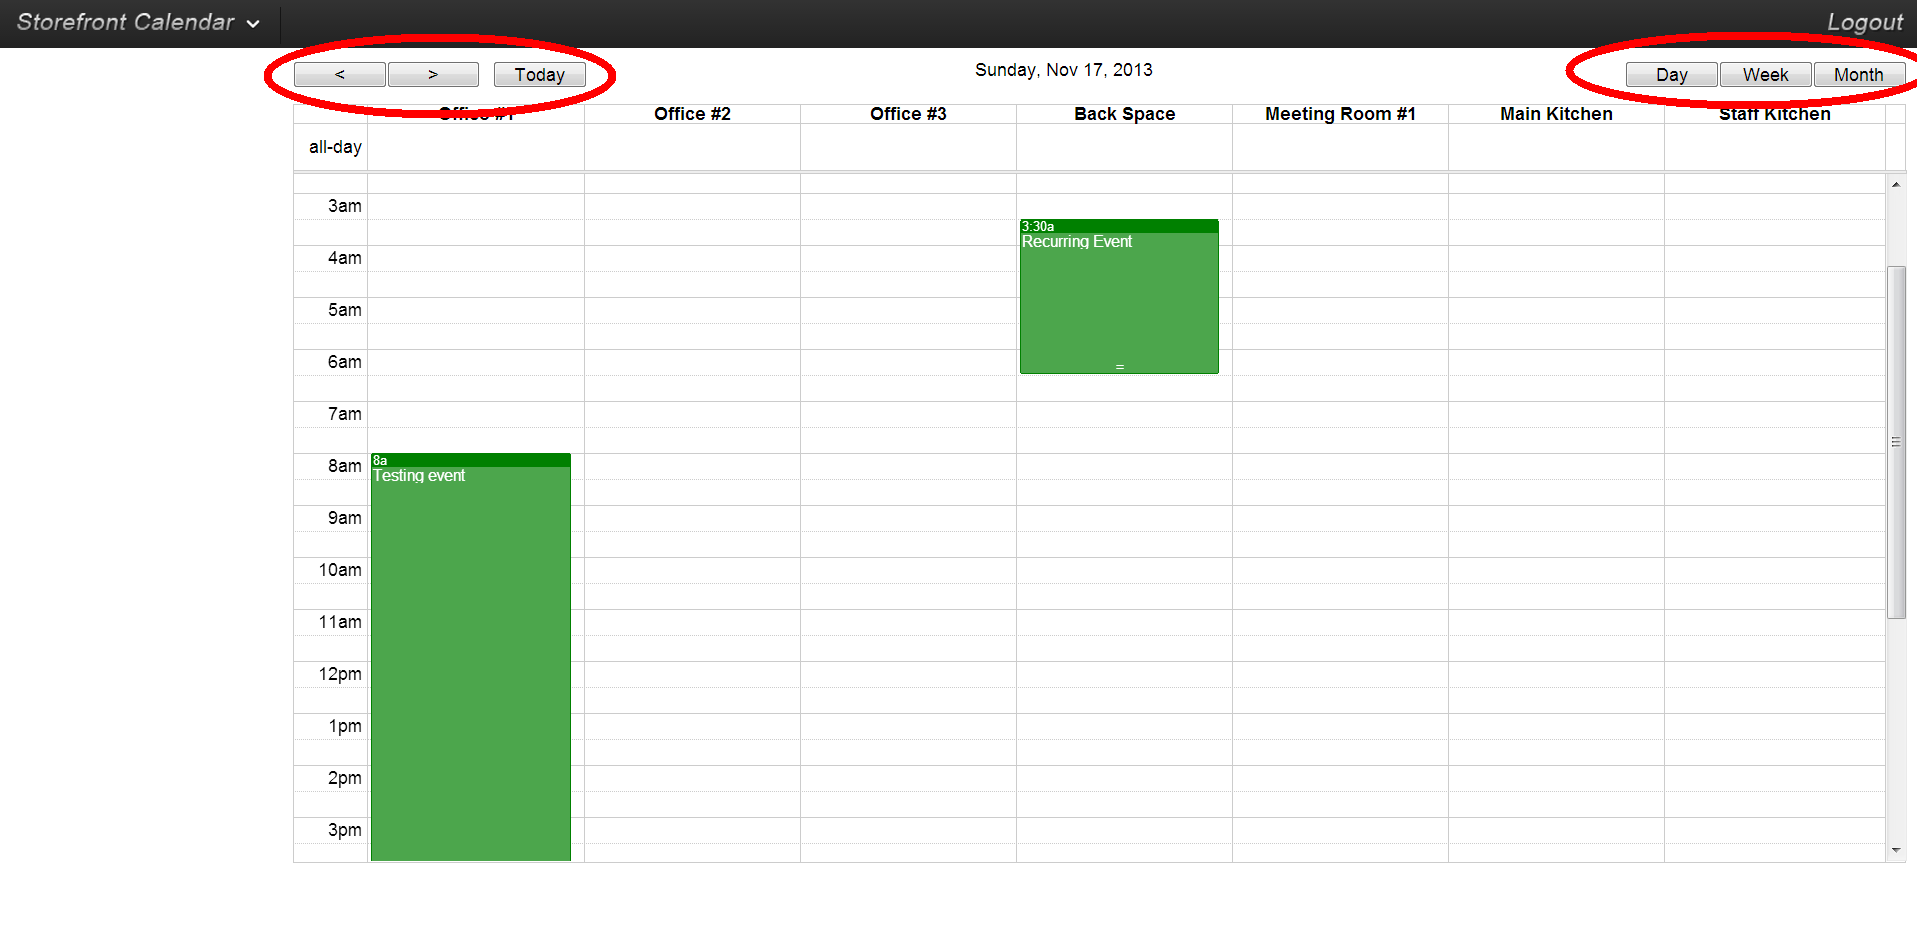
\includegraphics[width=\linewidth]{screenshots/img_day}



